\documentclass[aspectratio=169]{beamer}
\usetheme{Madrid}
\usepackage{graphicx}
\usepackage{booktabs}

\title{Branch Specialization in Attention}
\subtitle{Phase 0 Raw Attention-Score Stability Checkpoint}
\author{Research checkpoint}
\date{May 21, 2026}

\begin{document}

\begin{frame}
  \titlepage
\end{frame}

\begin{frame}{Current Question}
  \textbf{Core framing:}

  Does structural branch design in transformer-style architectures induce stable
  functional specialization or functional modularity across random seeds?

  \vspace{0.6em}
  \textbf{Phase 0 target:}

  Before training new architectures, verify that cross-seed attention-head
  similarity can be measured cleanly on existing multi-seed models.
\end{frame}

\begin{frame}{Method}
  \begin{itemize}
    \item Model: Pythia-160M, seeds 1--9, final revision \texttt{step143000}.
    \item Probe set: 8 short texts, max sequence length 64.
    \item Unit: layer-head attention matrix.
    \item Similarity: cosine similarity over valid causal token pairs.
    \item Alignment: raw same-index comparison and Hungarian-matched comparison.
    \item Null: random head permutation baseline within layer.
  \end{itemize}
\end{frame}

\begin{frame}{Key Aggregate Result}
  \begin{table}
    \centering
    \begin{tabular}{lrr}
      \toprule
      Metric & Probabilities & Raw scores \\
      \midrule
      Same-index mean & 0.7127 & 0.3735 \\
      Hungarian-matched mean & 0.8127 & 0.6692 \\
      Matched minus random mean & 0.0998 & 0.2982 \\
      Max layer-pair gap & 0.2272 & 0.7550 \\
      \bottomrule
    \end{tabular}
  \end{table}

  Raw pre-softmax scores are much more discriminating than returned attention
  probabilities.
\end{frame}

\begin{frame}{Raw Score Layer Profile}
  \centering
  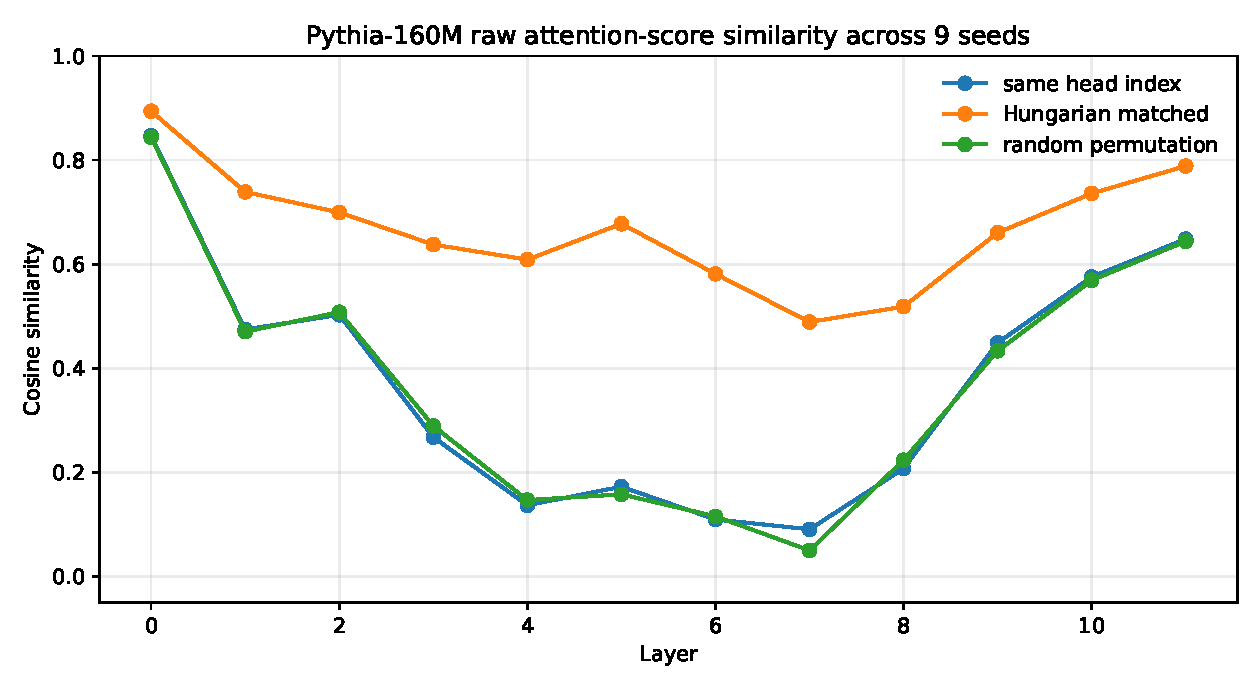
\includegraphics[width=0.88\linewidth]{figures/raw_score_layer_profile.pdf}
\end{frame}

\begin{frame}{Why Raw Scores Matter}
  \centering
  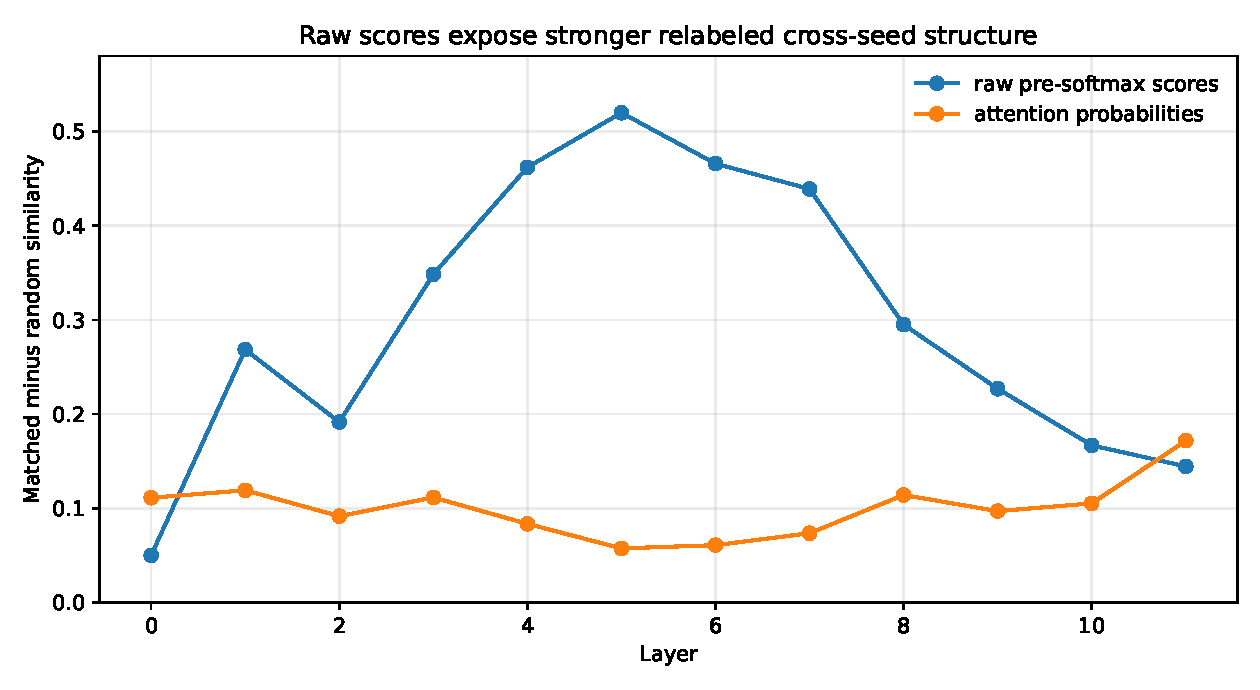
\includegraphics[width=0.88\linewidth]{figures/raw_vs_probability_gap.pdf}
\end{frame}

\begin{frame}{Interpretation}
  \begin{itemize}
    \item Same-index head stability is weak in many middle layers under raw-score comparison.
    \item Hungarian matching recovers substantially stronger cross-seed correspondence.
    \item This supports a weak-universality framing: similar attention-score roles emerge, but not reliably in the same head slot.
    \item Probability-space comparison appears too forgiving because softmax and generic attention patterns inflate similarity.
  \end{itemize}
\end{frame}

\begin{frame}{Caveats}
  \begin{itemize}
    \item This is still only attention-score behavior, not causal task specialization.
    \item The probe set is small and hand-written.
    \item The raw-score hook is currently implemented for GPT-NeoX/Pythia, not all model families.
    \item The next claim must use task-specific specialization scores, not attention similarity alone.
  \end{itemize}
\end{frame}

\begin{frame}{Decision}
  \textbf{Use raw pre-softmax attention-score similarity as the primary Phase 0 stability metric.}

  \vspace{0.8em}
  Keep probability-space attention similarity as a secondary sanity check.

  \vspace{0.8em}
  The next decisive experiment is to compute task-specific specialization
  \(S(h,t)\) for simple induction / previous-token probes and compare raw vs
  matched cross-seed consistency.
\end{frame}

\begin{frame}{Provenance}
  \begin{itemize}
    \item Script: \texttt{scripts/attention\_stability.py}
    \item Raw-score output: \texttt{results/phase0\_pythia160m\_seed1\_to\_9\_step143000\_raw\_scores}
    \item Probability output: \texttt{results/phase0\_pythia160m\_seed1\_to\_9\_step143000}
    \item Report: \texttt{doc/phase0\_pythia160m\_raw\_score\_pilot.md}
    \item Data copied into this deck folder under \texttt{data/}
  \end{itemize}
\end{frame}

\end{document}
